\begin{ex}
 (Mack) Os polígonos de k lados (k múltiplos de 3) que podemos obter com vértices nos pontos da figura, são em :
  \begin{center}
      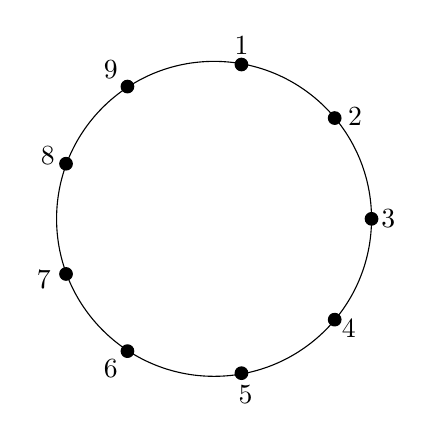
\begin{tikzpicture}
       \draw (0,0) circle [radius = 2];
       \draw [fill] (.348,1.96) circle [radius = .08];\node at (.348,1.96) [above] {1};
       \draw [fill] (1.532,1.28)  circle [radius = .08];\node at (1.58,1.3) [right] {2};
       \draw [fill] (-1.88,.7) circle [radius = .08];\node at (-1.9,.8) [left] {8}; 
       \draw [fill] (-1.88,-.7) circle [radius =.08];\node at (-1.95,-.77) [left] {7}; 
       \draw [fill] (.348,-1.96) circle [radius = .08]; \node at (.4,-2) [below] {5};
       \draw [fill] (1.532,-1.28) circle [radius = .08];\node at (1.5,-1.4) [right] {4};  
       \draw [fill] (2,0) circle [radius = .08];\node at (2,0) [right] {3};
      \draw [fill] (-1.1,1.68) circle [radius = .08];\node at (-1.1,1.9) [left] {9};
      \draw [fill] (-1.1,-1.68) circle [radius = .08];\node at (-1.1,-1.9) [left] {6};
      \end{tikzpicture}
  \end{center}
 
    \begin{enumerate}[(a)]
    \item 83
    \item 84
    \item 85
    \item 168
    \item 169
    \end{enumerate}
      \begin{sol}
       resposta: e \\
       $k=\{3,6,9\}\Longrightarrow \mathrm{C}_{9,3}+\mathrm{C}_{9,6}+\mathrm{C}_{9,9}=169$
      \end{sol}
\end{ex}